\documentclass[12pt, a4paper, oneside]{book}


%------------------------
% IMPORT PACKAGES
%-----------------------
\usepackage{amsthm}
\usepackage{mathtools}
\usepackage{algpseudocode}
\usepackage[chapter]{algorithm}
\usepackage{amssymb}
\usepackage{graphicx}
\usepackage{caption}
\usepackage{fancyvrb}
\usepackage{array}
\usepackage[gen]{eurosym}
\usepackage{cancel}
\usepackage{multicol}
\usepackage[acronym,toc,nohypertypes={acronym,notation},nonumberlist,automake]{glossaries}
%\usepackage{hyperref}
\usepackage{epigraph}
\usepackage{url}
\def\UrlBreaks{\do\/\do-}
\usepackage{breakurl}
\usepackage[breaklinks]{hyperref}

%% remark theoremstyle
%\newtheoremstyle{break}
%{\topsep}{\topsep}%
%{\itshape}{}%
%{\bfseries}{}%
%{\newline}{}%
%\theoremstyle{break}
%\newtheorem{remark}{Remark}[section]

% problem theoremstyle
%\newtheoremstyle{problemstyle}  % <name>
%{10pt}  % <space above>
%{10pt}  % <space below>
%{\normalfont} % <body font>
%{}  % <indent amount}
%{\bfseries\itshape} % <theorem head font>
%{\normalfont\bfseries:} % <punctuation after theorem head>
%{.5em} % <space after theorem head>
%{} % <theorem head spec (can be left empty, meaning `normal')>
%\theoremstyle{problemstyle}
%\newtheorem{problem}{Problem}[section] % Comment out [section] toremove section number dependence
%\newtheorem{definition}{Definition}[section]
%\newtheorem{theorem}{Theorem}[section]
%\newtheorem{proposition}{Proposition}[section]
%\newtheorem{remark}{Remark}[section]
%\newtheorem{lemma}{Lemma}[section]
% create command for variance in math mode
%\newcommand{\Var}[1]{\operatorname{Var}\left[#1\right]}
\newtheorem{mydef}{Definition}[section]
\newtheorem{myrem}{Remark}[section]
\newtheorem{myexample}{Example}[section]
\newtheorem{myprop}{Proposition}[section]
\newtheorem{mylemma}{Lemma}[section]
\newtheorem{mytheorem}{Theorem}[section]

\renewcommand\textflush{flushright}
\setlength\epigraphwidth{.6\textwidth}

\makeglossaries
\newacronym{}{}{}





\begin{document}


%----------------------------------------------------------------------------------------
% COVER PAGE
%----------------------------------------------------------------------------------------
\pagestyle{empty}
\begin{titlepage}

	\begin{center}
		\normalsize 
			\textsc{Politecnico di Milano}\\
			Scuola di Ingegneria Industriale e dell'Informazione\\
      		Corso di Laurea Magistrale in Ingegneria Matematica\\
	\end{center}
	\vspace{.6cm}
	
	\begin{figure}[htpb]
		\centering
		
\includegraphics[width=4cm]{Cover/polimi}
	\end{figure}
	\vspace{.6cm}
	
	\begin{center}
		\LARGE
			\textsc{Addressing Privacy and Fungibility Issues in Bitcoin: Confidential Transactions}
	\end{center}
	\vspace{1.6cm}

	\begin{flushleft}
		\large
		\begin{tabular}{ll}
		Relatori:    & Prof. Daniele MARAZZINA      \\
		             & Prof. Ferdinando Maria AMETRANO
		\end{tabular}
		\vspace{1cm}
	\end{flushleft}
	
	\begin{flushright}
		\large
		Tesi di Laurea di:\\
		Alessandro MIOLA\\
		Matr. 862753\\		
	\end{flushright}
	
	\vspace*{\fill}
	\begin{center}
		Anno Accademico 2017-2018
	\end{center}
	
\end{titlepage}


%----------------------------------------------------------------------------------------
% ABSTRACT
%---------------------------------------------------------------------------------------

%% Set page numbers of the introduction to roman  
\frontmatter
\pagestyle{plain}
%\chapter{Abstract}
\label{chpr:abstract}
Insufficient privacy is recognized to be one of the major vulnerabilities of the Bitcoin's protocol, even because it undermines its fungibility. Bitcoin eliminates the need for a trusted third party, but mainly faces users' privacy by hiding them behind pseudonymous addresses.\\
This work aims at presenting \textit{confidential transactions}, the first proposal for a transaction format with encrypted amounts in Bitcoin, which would strongly increase value privacy. It exploits homomorphic encryption which does not remarkably hurt universal validation of transactions, a crucial premise for the achievement of a distributed consensus on the order of valid transactions.

%\cleardoublepage
\vspace*{\fill}
\epigraph{\textit}{}{}
\vspace*{\fill}


%----------------------------------------------------------------------------------------
%	LIST OF CONTENTS/FIGURES/TABLES PAGES
%----------------------------------------------------------------------------------------

\tableofcontents
\listoftables
\addcontentsline{toc}{chapter}{List of Tables}
\listoffigures
\addcontentsline{toc}{chapter}{List of Figures}
\listofalgorithms
\addcontentsline{toc}{chapter}{List of Algorithms}
\printglossaries

\chapter{Abstract}
\label{chpr:abstract}
Insufficient privacy is recognized to be one of the major vulnerabilities of the Bitcoin's protocol, even because it undermines its fungibility. Bitcoin eliminates the need for a trusted third party, but mainly faces users' privacy by hiding them behind pseudonymous addresses.\\
This work aims at presenting \textit{confidential transactions}, the first proposal for a transaction format with encrypted amounts in Bitcoin, which would strongly increase value privacy. It exploits homomorphic encryption which does not remarkably hurt universal validation of transactions, a crucial premise for the achievement of a distributed consensus on the order of valid transactions.
\chapter{Acknowledgements}
\label{chpr:acknowledgement}
First of all, I would like to thank my thesis supervisors: Prof. Ferdinando Ametrano for having shared his passion for the subject and knowledge with me and Prof. Daniele Marazzina for his precious advices during the drawing up phase.\\ \ \\
Then, I would like to express my profound gratitude to my parents and Albi for having always been by my side: mum, for for having taught to me that gentle manners always win, for her sensibility and for being mum (it is difficult to say it otherwise!); dad, for having wisely taught to me that anything can be reached with commitment and determination and for all the efforts spent in helping me become a better man; Albi for having turned bad days with a smile or a joke. And a big thank goes to my grandparents too, for having always supported me despite the distance.\\ \ \\
Furthermore, I would like to thank my high school friends. Having encountered all of you has been a great gift. In particular, Gio (the nicest man I know), the great Lollo and the wise Luca. And again Ambra, Anna, Chiara, Cicchi, Genna, Marti, Massi, Miks and Ventu.\\ \ \\
Finally, a special thanks also goes to the great friends met at university. First of all to Dodo, Gallo, Gigi, Giulio, Gugo, Michi, Simo and Teo. These years would have been even harder without you. And again to Antea, Pietro, Richi and many others I had the opportunity to meet and work with.\\ \ \\
Thank you all.



%----------------------------------------------------------------------------------------
%	THESIS CONTENT - CHAPTERS
%----------------------------------------------------------------------------------------

\mainmatter

\chapter{Introduction}
\label{chpr:intro}

\section{Structure}

\chapter{Privacy and fungibility issues in Bitcoin}
\label{chpr:priv_fung}
Traditional, centralized financial institutions provide a level of privacy in their systems with respect to the outside world which is necessary for personal and commercial reasons at first (to preserve the freedom to transact, not to let commercial competitors monitor your own activity). The obvious concern, however, is that this level of privacy is not guaranteed against the same institutions providing the service and this opens a lot of issues regarding data collection and data privacy. \\
Bitcoin's breakthrough to have succeeded in building a decentralized distributed network where distributed consensus is reached among the nodes of the network has put some constraints on the underlying security model which seem to conflict with the privacy issues addressed above. However this is quite unavoidable: whereas decentralized systems are easy to build without consensus and, on the other hand, consensus is easy to achieve in centralized systems, maintaining both properties in the same system proves to be a hard challenge.\\ 
Bitcoin's security model is based on the achievement of distributed consensus which in turn requires (among the others) universal and independent verification of the validity of each transaction, made possible by having public transaction data. That is, transparency is needed to obtain and strengthen security.\\
This lack of privacy is recognized to be a weak point within the Bitcoin's protocol and several proposals to improve different aspects of privacy in Bitcoin have appeared in the years, despite never being effectively softforked. The main reason for this being basically the high costs that the massive adoption for privacy-based solutions would imply: privacy is costly and requires commitments. Nevertheless, advances in monitoring capabilities of the blockchain, newborn businesses in Bitcoin blockchain's analysis urge the need for privacy-based solutions in the long run.\\
The original protocol has addressed the problem mainly through the adoption of pseudonymous addresses, that on one hand seem robust if one does not know who owns which addresses, but suffer both from some unsafe users practices (like address reuse) and from the possibility to exploit coins linkability\footnote{The need of a user to generally spend the change back to himself when transacting (due to transaction outputs generally not embedding the right value to be spent in a successive transaction) basically links transaction outputs and so addresses. Moreover in case previously collected changes are too small to cover a transaction output in its entirety, this makes it necessary to combine changes and so further linking transactions.} to trace the transaction graph.\\
Instead, a point in favour of having less privacy and more transparency comes from whom is mainly concerned with the use of cryptocurrencies like bitcoin for illicit activities, who argues that this could be a feature that can help investigations.
\section{Types of privacy in Bitcoin}
\label{sec::priv_1}
Due to how the Bitcoin's protocol has been conceived and implemented, the aim to strengthen privacy should regard different aspects whose improvement can be beneficial. In particular, the concern should be at least on \textit{association} privacy, \textit{balance} privacy, \textit{identity} privacy and \textit{transaction value} privacy.\\
Improving association privacy would mean enhancing transaction graph privacy not letting the possibility to understand who is paying who, thus addressing the previously discussed linkage between transactions and making transaction graph analysis harder. A typical practice undermining it is address reuse, that is however nowadays reduced by wallets using a Hierarchical Deterministic derivation of keys (and so addresses). Moreover, different solutions have been proposed in this field in the years. We present the idea behind only some of them, but it is worth to notice that solutions trying to address association privacy are many more.\\ One of the first is Coinjoin \cite{Max13}, which starts from the important premise that when a transaction spends from multiple addresses it is not necessarily the case that these addresses all come from the same party, but instead people could eventually cooperate to agree on a set of inputs to spend and a set of outputs to pay to and individually sign their own inputs only. On top of this it even exploits the absence of a mapping between inputs and outputs in a transaction or better the \textit{many-to-many} mapping existing between them (in a transaction with more than one input, it is not possible to say which input ends up being which of the outputs or which part of) to create a single transaction jointly authored\footnote{All of the transaction inputs are shuffled among several participants, each signing their inputs only.} by several participants in such a way that they do not have to trust each other. Indeed, each participant is only signing his own inputs (thus making it unnecessary to know who other is involved in the coinjoin) and it is the case that if some of the inputs are not signed the transaction would be invalid.\\
Observe moreover that the users involved in the coinjoin would even agree on a uniform output size and on burning inputs of at least that size. Indeed, unless all of them trading to the same amount it would be easy to discover the correlation between inputs and outputs.\\ 
Another solution which even provides association privacy, although was not born primarily for this purpose, is certainly Lightning Network \cite{RefWork:18}, whose gain in transaction graph privacy derives for instance from the possibility of the parties taking part to a multi-hop channel to basically transact without sending data to the blockchain. \\ 
Improving balance privacy, instead, should aim at protecting against the possibility of deducing the balance of a wallet. Thus it is somehow linked to achieving association privacy.\\
Achieving identity privacy refers to the possibility of each user to prevent his identity to be associated with the coins. Identities could be at risk first of all because Internet itself is not really identity preserving (and not very anonymous); many services such as exchanges or on-line stores accepting bitcoins generally require and have access to personal information (credit card or bank account details, shipping addresses, IP addresses and so on).\\
The last privacy aspect which deserves credit is transaction value privacy, which actually is the main concern of the Confidential Transactions \cite{Max15} solution. The idea is to protect against other people knowing the value of everyone's transactions, which is kind of standard for traditional financial services. That is, it affects the \textit{confidentiality} Bitcoin transactions lack at all. Some concrete examples could stress the need for such improvements. For instance, a common implication for employees of a company paying wages in bitcoin is that they'll have their wages public, which is not that nice. Another possible example where amount privacy turns out to be necessary, though less conflicting common bitcoins' owners, configures when somebody's wallet spends a large sized input for a small payment, thus paying back to itself a high change; in this case, the possibility of being targeted for theft would be at least real.\\
As a final and general note, it should be observed that we have just described a few of the bunch of proposals that could help achieving better privacy in Bitcoin and in particular we have considered the proposals more closely related to the addressed one. But, for instance, it is worth mentioning the impact that the introduction of Schnorr signatures \cite{Schnorr} would have on privacy in Bitcoin mainly through signatures aggregation (even across signers), which is obtained by exploiting the linearity property of the Schnorr scheme.

\subsection{Confidential transactions address value privacy}
\label{sec::CT_value_priv}
Confidential transactions is the first and only solution addressing value privacy in the Bitcoin ecosystem. All previous solutions mainly addressed association privacy. However, as well explained by Bitcoin Core developer G. Maxwell,\footnote{During a conference whose video is available at \url{https://www.youtube.com/watch?v=LHPYNZ8i1cU}.} there should be a broader awareness on issues related to value privacy. For instance in the comparison with the Internet protocols, providing association privacy means anonymizing the identity of people communicating, which is not much of a worry unless for people using Tor. On the other hand, what people worry about is making the content of communications private, which is what value privacy effectively provides.\\
The way confidential transactions achieve value privacy is by encrypting the transaction amount (which is instead available in the clear in a standard Bitcoin transaction) and more precisely they exploit homomorphic encryption\footnote{More details will be available in the next chapters.} to preserve the ability of the network to verify and validate transactions.\\
It should be noticed that confidential transactions only provide value privacy, not affecting transaction linkability, but they naturally integrate with various proposals addressing association privacy.

\subsection{Compatibility with different solutions}
\label{sec::compatibility}
As mentioned, it turns out that confidential transactions can not only integrate previous solutions addressing association privacy, but also help in solving some of their problems. In particular 
we focus again on the relation with Coinjoin \cite{Max13}, bearing in mind that most of the following arguments are even valid for similar proposals\footnote{E.g. Coinswap or Tumblebit.}.\\
We have briefly described how Coinjoin works, but we have not focused yet on all of its limits. The first one is certainly coordination between users: it is not that easy to find people agreeing on transacting at the same time and for the same exact amount. The second one was briefly addressed above and it is basically the fact that Coinjoin achieves some sort of privacy provided that input and output values are somehow matching.\\
If we integrate with confidential transactions some of the previous issues disappear because having amounts encrypted prevents from the necessity to mix inputs of almost the same size to pay to outputs of the same size, while taking the advantage of achieving association privacy.

\section{Fungibility}
It turns out that fungibility is quite relevant in this discussion. Thus, we can start explaining what fungibility is. Fungibility is the property of a unit of a good to be completely indistinguishable from any other unit of the same good (or at least treated as such) and consequently completely interchangeable. To give some examples, diamonds are not completely fungible\footnote{Gold is much more fungible.}: little differences in their properties (cut, hardness, color etc.) make it difficult to find diamonds expected to be equally valued. Another possible example of non-fungible good is a piece of art as it is clearly not possible to exchange one for one other.\\
For what concerns currencies, fungibility is a crucial property: we do not want to care of receiving a physical banknote being worth less than a different banknote of the same denomination nor we want to care of the possibility of the possession of this same banknote being revoked as it was involved in a robbery some transactions ago.\footnote{Though observe that even \euro{} or US\$ or most of the other currencies are not completely fungible, they have serial numbers, but we basically treat them as such because non-fungible solutions for currencies wouldn't work.} The possibility of blacklisting physical banknotes, other than being quite unfeasible, would destroy confidence in receiving them, thus impacting the whole economy. And actually that's not just a matter of practice but has been established by law. Differently from a stolen piece of art, whose possession would be revoked in the same moment of the discovery, that would not be ever the case for physical banknotes in most countries of the world.
\subsection{Bitcoin is weakly fungible}
\label{sec::weak_fun}
When speaking of fungibility, what makes discussion on Bitcoin intertwine and compare with that on money in its cash-like forms, rather than with that on its inter-mediated means of payment is Bitcoin's peculiarity to be (substantially) immediate and final payment, exactly like cash. Moreover, inter-mediated means of payment compromise some desirable features of money (among which fungibility itself).\\
Bitcoin turns out to be weakly fungible, which is the other recognized weak point of the protocol. The main reason for it should be found, again, in the transparency of the blockchain (feature and bug), which makes it possible in principle to trace the provenance of every coin and so discern between them. What actually happens is on one side to have some coins which are worth more than others,\footnote{Think of freshly minted coins that, being ``clean", can be traded for a higher premium.} the ones with less value becoming the preferred ones to be exchanged; on the other side, the growth of businesses specialized in the analysis of the transactions flows on the blockchain might turn somebody unwilling to accept certain coins further or exchanges to freeze accounts just for the ``bad history" of a coin.\\
Lack of fungibility could even have more risky consequences for Bitcoin itself. It can jeopardize its permissionless nature because receiving coins and be prevented from spending can make users doubt of whether it's safe to receive and in turn can make them begin to consult blacklist services before transacting again. Or it can lead to a generalized loss of confidence which would make prices drastically decline.\\
As a side note, it should be said that there have been in time various proposals to create services to register Bitcoin users (kind of blacklisting services) and among the invoked reasons behind their possible adoption was always the idea of reducing Bitcoin-related crimes. However, it is likely that criminals already circumvent the regulated exchanges when buying or selling bitcoins, thus being probably not affected.\\
Based on the described picture it is evident that the same aspects making Bitcoin non-private make it also non-fungible.\\
Thus among the solutions favouring fungibility we can include the same privacy-based solutions outlined before. Then, another important aspect fungibility benefits from is mining decentralization\footnote{Though note that mining in Bitcoin is quite centralized.} which guarantees that sooner or later a user's transaction will be processed and mined without miners discriminating between coins in the act of processing transactions.
\subsection{Fungibility vs scalability}
\label{sec::fun_vs_scala}
Scalability is another highly debated aspect in Bitcoin. It refers to the possibility of increasing the transaction capacity, making the network able to process more transactions per second. In particular, it is in the comparison with centralized payment solutions, such as Visa, that the discussion gets going. The reality is that, by design, Bitcoin is not suited to process the volume of transactions of a centralized circuit like Visa\footnote{According to \url{https://usa.visa.com/run-your-business/small-business-tools/retail.html}, Visa can be able to process 24000 tps at its peak, Bitcoin only 7 tps.} and this for simple reasons: each transaction in Bitcoin is broadcast to and through all of the nodes of the network, each of whom has to keep an updated copy of the entire ledger of transactions; centralized solutions on the other side only require a centralized ledger to which all transactions are committed and a few backups. If Bitcoin processed the same number of transactions of the Visa circuit this would result in a bloat of the blockchain size, running totally outside the realm of processing power of available computers. \\
Moreover, scalability in Bitcoin is also affected by transactions confirmation being slow and probabilistic compared to centralized systems, where confirmations happen in fractions of a second.\\ Thus, it is likely that higher scalability will mainly come through off-chain solutions exploiting the blockchain for verification of balances (and settlement of disputes, see e.g. \cite{RefWork:18}) rather than transfers.\\
Far from being a discussion on scalability issues and proposed solutions, this paragraph only wants to briefly investigate the connection between fungibility (and privacy) on one side and scalability on the other side. Indeed, the described expensive nature of privacy-based solutions generally put fungibility and scalability in a seemingly insurmountable trade-off. However, there are situations where fungibility helps scalability: the reduction of information leakage (in particular that information enabling transactions to be linked and reducing anonymity) would potentially help scalability by preventing relevant information to go and appear in the blockchain. Mimblewimble \cite{MW} is an example of an application that provides privacy and fungibility (mainly through the adoption of confidential transactions) but even achieves better scalability than Bitcoin by the possibility to remove most of historic data by pruning spent transaction outputs and possibly validating the whole history without downloading these already spent transactions.\\
Conversely, having a more scalable network would obviously favour fungibility and let open the possibility to exploit more expensive privacy-based solutions, but it is indeed difficult to achieve.
\chapter{Cryptographic primitives}
\label{chpr:crypto_primitives}
In this section we present the cryptographic primitives which are necessary to build a \textit{confidential transaction}.\\
Prior to this, however, we start with a crash dive into some pillars of Elliptic Curve Cryptography (ECC), the focus being just on what can be useful to follow the incoming narration. We refer, instead, to \cite{Sec} or \cite{UnderstandingCrypto} for a more deep approach.\\
Elliptic Curve Cryptography is a public-key cryptosystem built on elliptic curves defined over finite fields and, for our purposes, it is the cryptosystem Bitcoin uses to secure the transactions. It is based on the intractability of the Elliptic Curve Discrete Logarithm Problem (ECDLP), namely the infeasibility of computing the discrete logarithm of a random elliptic curve point with respect to a publicly known base point\footnote{At the base of public-key cryptography there is always the intractability of a particular mathematical problem: \begin{itemize} \item RSA public-key schemes: hardness of factoring large integers. \item DLP-based public-key schemes: hardness of solving the discrete logarithm problem. \item ECDLP-based public-key schemes: hardness of solving the generalized discrete logarithm over an elliptic curve. \end{itemize}}. The benefits over its prior alternatives (in the field of public-key or asymmetric cryptography) come from the possibility of providing the same security level with shorter operands, which is in turn a consequence of the problem being harder to solve. Indeed, it is even the latest solution which has come out among the mentioned alternatives.\\
Referring to the Appendix \ref{app:A} for both the definition of finite field (and how to get to it) and the presentation of the DLP (in its non-elliptic curve formulations) to avoid making this introduction unintentionally cumbersome, we give instead here the definition of \textit{elliptic curve} and we present the known translation of the DLP over elliptic curves (ECDLP).\\ 
The need to introduce elliptic curves is motivated by the necessity of searching a cyclic group where to build the cryptosystem\footnote{see DLP arguments in \ref{DLP} for more details.}; observe, however, that the mere existence of a cyclic group is not sufficient, the problem being to find such one where the DLP is computationally hard to solve. It turns out that elliptic curves are fitted for the purpose and thus the goal becomes to find elliptic curves with a large cyclic group. Later in this section, a theorem will support the suitability of elliptic curves in providing such a result, thus explaining their fundamental role in the discussion.\\
As remarked within the Appendix \ref{app:A}, for cryptographic use, the focus is just on elliptic curves defined over a finite field (in particular we consider $K = \mathbb{F}_p$, the finite field with p elements) rather than over generic fields (the set $\mathbb{R}$ being an example).
\begin{mydef}
\label{def_EC}
    The elliptic curve over $\mathbb{F}_p$\footnote{which we denote by $E(\mathbb{F}_p)$.} is the set of all pairs $(x,y) \in \mathbb{F}_p$ such that $\{(x,y) \in \mathbb{F}_p \times \mathbb{F}_p: y^2 = x^3 + ax+b \mod p\} \cup \{\infty\}$ with $a,b \in \mathbb{F}_p$ and such that the consistency condition $4 a^3+27b^2 \neq 0 \mod{p}$ holds true.
\end{mydef}
\noindent
The problem now becomes both identifying the group elements and defining a group operation with these elements. Group elements are nothing else than the points fulfilling the curve equation in \ref{def_EC}, the definition of the group operation is not presented here, for the details we refer to \cite{UnderstandingCrypto}.\\
The only point we want to stress is the meaning of $\{\infty \}$ in definition \ref{def_EC}:
\begin{myrem}
    $\{\infty \}$ is the so called infinity point and turns out to be the identity element of the group defined by the points over the elliptic curve together with its group operation.
\end{myrem}
\noindent
At this point, it is possible to state the following theorem, which eventually closes the circle by explaining the reason why it is possible to build a DLP with elliptic curves.
\begin{mytheorem}
    The points on an elliptic curve, together with the infinity point $\{\infty \}$ (other than defining a group by themselves once the group operation is defined) have cyclic subgroups. Moreover, under certain conditions (merely if the group order is prime) all points on an elliptic curve form a cyclic group.
\end{mytheorem}
\begin{myrem}
    By specializing the notation seen in the Appendix \ref{app:A} to the EC case, we denote by $G$ the generator of a cyclic (sub)group defined over an elliptic curve (being an element of the (sub)group itself, it is nothing else than a point on the curve). Thus, starting from $G$ it is possible to explore the entire (sub)group (thus recovering all the (sub)group points) by repeatedly applying the group operation to $G$.
\end{myrem}
\begin{myrem}
    If the EC (sub)group has order $m$, the application of the EC group operation $m$ times gives back the identity element of the EC group.
\end{myrem}
\begin{myrem}
    If the EC group order n is prime, any point of the curve is a generator $G$. This basically comes from \ref{thm::prime_order_all_gen}.
\end{myrem}
\noindent
With this theoretic framework at our disposal, we can conclude the introduction to this chapter by presenting the ECDLP.
\begin{mydef}
    Given the elliptic curve $E(\mathbb{F}_p)$ with generator $G$, consider another element of the curve, $Q$. The ECDLP is finding the integer $q, 1 \leq q \leq \#E(\mathbb{F}_p)$, such that $\underbrace{G+G+\dots+G}_{q \quad times}$=$qG$=$Q$.
\end{mydef}
\noindent
For what concerns notation, in ECC $q$ is the \textit{private key}, which is an integer, while $Q$ is the \textit{public key}, a point on the curve with coordinates $(x_Q, y_Q)$.

\section{Commitment schemes}
\subsection{Additively homomorphic commitment}
\subsection{Pedersen commitment}
\section{Zero-Knowledge Proofs of Knowledge}
\section{Ring signatures}
\section{ECDH}
The elliptic curve Diffie-Hellman primitive is a cryptographic primitive which is at the basis of the ECDH Key Exchange scheme.\\
In turn, the elliptic curve Diffie-Hellman Key Exchange (ECDH) is a key agreement scheme based on ECC, thus relying on the hardness of the ECDLP. It is the EC counterpart of the well known\footnote{in cryptography at least.} Diffie-Hellman Key Exchange (DHKE) protocol. In this section we just present the scheme for the elliptic curve version.\\
It allows two entities, both endowed with an elliptic curve private-public key pair, to engage in a key agreement scheme and establish a shared secret over an insecure (yet authenticated) channel. The shared secret can then be both used directly as key or as seed to derive other key(s), for instance (but it is just a possibility) via a deterministic generation procedure like RFC6979 (see \cite{rfc6979}).
\subsection{ECDH primitive}
The primitive is built in such a way that both the parties by means of one of their own private key and one of the public key of the other party can recover, autonomously, the same (shared) secret.\\
Here how's the primitive built. Suppose Alice and Bob want to establish a shared secret. The primitive is run autonomously by both and takes as input valid elliptic curve domain parameters $T$\footnote{$T$ = $(p, a, b, G, n, h)$; $p$ specifies the prime finite field $\mathbb{F}_p$; $a,b \in \mathbb{F}_p$ are the coefficients of the elliptic curve equation; $G \in E(\mathbb{F}_p)$ is the elliptic curve generator point; $n$ is the order of $G$, that coincides with the number of points of the cyclic subgroup generated by $G$; $h = \#E(\mathbb{F}_p)/\ n$ is the so called cofactor.}, a private key owned by who is running the procedure ($q_A$ for Alice, $q_B$ for Bob) and the public key corresponding to the other party private key (Alice takes $Q_B$=$q_BG$ as input, Bob takes $Q_A$=$q_AG$ as input\footnote{though, Alice does not obviously know $q_B$, nor Bob $q_A$.}). The output is a shared secret field element $z$ or the string ``invalid" otherwise.\\
The algorithm below refers to the generation of the shared secret from Alice. The same can be done for Bob, by carefully exchanging the roles of the parameters.
\begin{algorithm}
	\caption{ECDH primitive}
	\label{alg:ECDH}
	\begin{algorithmic}[1]
		\Procedure{ecdh}{$T, \ q_A, \ Q_B$}
		\State $S = (x_S,y_S) \gets q_AQ_B$
		\State assert $S \neq \{\infty\}$
		\If {$S = \{\infty\}$}
		\State \textbf{return} ``invalid"
		\EndIf 
		\State \textbf{return} $z \gets x_S \mod{n}$ 
		\EndProcedure
	\end{algorithmic}
\end{algorithm}\\
It turns out to be straightforward to prove that the shared secret computed by both parties is the same. Alice: $q_AQ_B = q_A(q_BG)$; Bob: $q_BQ_A = q_B(q_AG)$ $\rightarrow$ by associativity of the group operation (point addition), the result holds and both compute $S=q_Aq_BG$.
\subsection{ECDH Key Exchange protocol}
According to notation in \cite{Sec}, the key exchange protocol involves a \textit{setup} phase, a \textit{key deployment} procedure and a \textit{key agreement} operation (which actually exploits the ECDH primitive).
Here's a simple graphical representation of the key exchange protocol combining the key deployment phase (in its associated public keys exchange phase) and an instance of the ECDH primitive explained above.
\begin{center}
	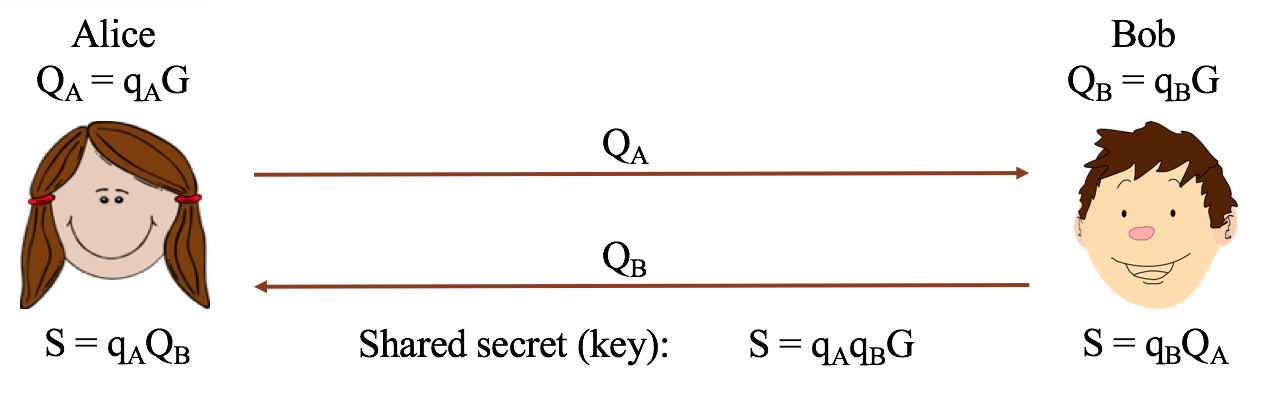
\includegraphics[scale = 0.55]{Images/ECDH.png}
	\captionof{figure}{ECDH key exchange}
	\label{fig:ECDH}
\end{center}
The \textit{setup} phase defines the choice of the elliptic curve domain parameters.\\
The \textit{key deployment} phase requires both parties establishing valid private-public key pairs $(q_A,Q_A)$, $(q_B,Q_B)$ and exchanging their public keys $Q_A$ and $Q_B$ (with further assurance of the public keys being valid ones).\\
The \textit{key agreement} operation defines a way to obtain shared keying data from a shared secret by means of a suitable key derivation function. Observe, however, that the keying data might not directly be used as a key, this just depends on the application.\\ The algorithm below refers to the generation of the shared key by Alice. Bob's algorithm is straightforward and just requires rearrangement of the parameters. We first describe the key derivation function (KDF), taking as inputs an octet\footnote{to keep it simple we can consider an octet being equivalent to a byte.} string $Z$ derived from the field element $z \in \mathbb{F}_n$ outputted by the ECDH primitive\footnote{for more details on the \textit{field-to-octet} conversion, see \cite{Sec}.}, the integers \textit{keydatalen}, \textit{hashlen}, \textit{hashmaxlen} which refer to the length in octets respectively of shared key, hash values and maximum lenght of messages that can be hashed with the given hash function. It outputs a shared key $K$ (octet string) or ``invalid". 
\begin{algorithm}
	\caption{Key Derivation Function}
	\label{alg:KDF}
	\begin{algorithmic}[1]
		\Procedure{kdf}{$Z, \ keydatalen, \ hashlen, \ hashmaxlen $}
		\State assert $|Z| + 4 < hashmaxlen $, ``invalid"
		\State assert $keydatalen < hashmaxlen * (2^{32} -1) $, ``invalid"
		\State $count \gets 1 $  \Comment{4 octet, big-endian string}
		\For {$i\gets 1, \lceil{keydatalen /\ hashlen}\rceil$}
		\State $K_i \gets hash(Z||count)$
		\State $count \gets count + 1$
		\State $i \gets i + 1$
		\EndFor
		\State $K \gets K \verb|>>=| (keydatalen - hashlen)$ \Comment{leftmost keydatalen octects of $K_1||\dots||K_{\lceil{keydatalen /\ hashlen}\rceil}$}
		\State \textbf{return} $K$ 
		\EndProcedure
	\end{algorithmic}
\end{algorithm}\\
Thus, the whole key agreement operation requires deriving a shared field element $z \in \mathbb{F}_n$ by running an instance of the ECDH primitive, converting it to an octet string to give as input to the KDF and consequently deriving a shared key.\\
For what concerns security arguments, it is required the ECDHP (elliptic curve Diffie-Hellman problem) to be hard to solve. It comes out it is closely related to the ECDLP, a third party willing to break it has to solve either $q_A = \log_G{Q_A}$ or $q_B = \log_G{Q_B}$. Consequently, provided a care choice of the parameters during the setup phase, the more powerful algorithms to break it are basically the same presented above for the ECDLP ($\sim O(|\mathbb{G}|^{\frac{1}{2}})$ steps). What that means practically is that with an elliptic curve group order higher than $2^{160}$ (i.e. $160$ bits)\footnote{bearing in mind that, as a rule of thumb, security levels of more than 80 bits are considered satisfactory.} the ECDHP wouldn't be possibly broken.\\ 
Then, another important security assumption relies on the so-called channel authentication for public key exchange, required to prevent \textit{man-in-the-middle} attacks. The latter consist in an adversary eavesdropping over the channel and substituting Alice and Bob's public keys with his own public keys. If the channel is not authenticated\footnote{where authentication means that the recipient has strong reasons to believe that the communication is in place with the ``designated" sender and can be achieved by means of some protocols we do not present here.}, this would prevent Alice and Bob being aware of sharing a secret with the eavesdropper rather than themselves.
%\chapter{Conclusions}
\label{chpr:conclusions}
This thesis has tried to motivate the importance for Bitcoin to adopt technologies enhancing privacy in the incoming years. This would not merely improve the privacy of people transacting (which is indeed fundamental), but even strengthen its ability to serve as money. Indeed, though it cannot be recognized as a good unit of account, Bitcoin is a good store of value (it is durable, it can be reliably saved, stored with low costs and easily retrieved) and an excellent medium of exchange (it is easily portable, divisible, swappable, resistant to counterfeiting). Its greatest lack is that it is not that fungible and it is the case that fungibility is strictly linked to privacy.\\
At the same time, this work should have outlined the reasons why no privacy-based solutions have been soft-forked yet in Bitcoin at the time of writing; this is not certainly for a lack of proposals, quite the opposite. Developers have worked in this direction since long time, but cryptographic, privacy-based solutions are costly and require commitments, thus opening other issues.\\
Moreover, through confidential transactions \cite{Max15} we have explored some nice features of homomorphic encryption applied to commitment schemes, the interesting field of Zero-Knowledge proofs, a fancy variant of digital signature scheme and a clever solution for the communication of transaction amount, blinding factors and other user-selected metadata between participants in the transaction.\\
Confidential transactions basically hides each output amount through a Pedersen commitment to the amount and add a range proof ensuring that the amount does not overflow. The solution we have described builds each range proof through a Borromean ring signature. Among the strengths of confidential transactions, the fact that these can be possibly constructed without new cryptographic assumptions with respect to the main protocol, but relying on the hardness of the ECDLP (differently from some alternative schemes like Zcash's ones) and the substantial savings in terms of size and verification time with respect to previous solutions (which have made them sources of inspiration for privacy-based alt-coins like Monero, that has effectively implemented confidential transactions through ring signatures, RingCT \cite{RingCTMonero}). On the other hand, the solution suffers from the size of the range proof attached to each transaction output (and thus of the entire transaction) being too large.\\
These weaknesses have prevented confidential transactions to be soft-forked in Bitcoin up to now.\\
More recently, however, a new and more efficient solution to range proof construction \cite{Bulletproofs} has been proposed. Its name is Bulletproofs and it is likely worth studying: it could be the solution being effectively soft-forked in the future (it even naturally marries some older proposals) and effectively bringing consistent privacy in the protocol. Indeed, Bulletproofs is still well-suited for constructing efficient range proofs on committed value, but it also adds various optimizations.\\
At first, it provides aggregation of range proofs: it would be possible to prove that $m$ commitments lie in a given range by just providing additional O($\log m$) group elements with respect to a single proof, making it growing logarithmically with the number of transaction outputs. This would be already useful for confidential transactions by themselves as standard Bitcoin transactions have generally at least two outputs and it would even make it efficiently combine with Coinjoin \cite{Max13}. Additionally it could simultaneously double the range proof precision at marginal additional cost.\\
Then, it would allow batched verification of multiple Bulletproofs.\\ All of these enhancements with a total transaction size not so bigger than a standard transaction according to \cite{Bulletproofs,CT_eff}.\\
Moreover, confidential transactions are even beneficial for a newborn and promising cryptosystem called Mimblewimble \cite{MW, PoeMW}. Mimblewimble is still a transaction output based system (thus a Bitcoin-like blockchain system) which however implements confidential transactions from the beginning. At the time of writing it is already being built through Bulletproofs, thus inheriting its benefits. Moreover, Mimblewimble removes the need for the unlocking script because it allows to prove a transaction to commit to a Pedersen commitment to 0 just signing the transaction through the difference of the commitments to outputs and inputs. Other than this, it can benefit from transaction aggregation and enables the construction of a simplified blockchain where spent transactions can be pruned, thus improving scalability.



%----------------------------------------------------------------------------------------
%	THESIS CONTENT - APPENDICES
%----------------------------------------------------------------------------------------

\appendix
\chapter{Abstract algebra fundamentals}
\label{app:A}
This appendix is aimed at providing some fundamental notions of  algebra of sets and number theory at the basis of the considered public-key cryptosystem. Definitions are mainly taken from \cite{UnderstandingCrypto} and adapted when needed.
\section{Groups}
We start from the definition of a \textit{group}.
\begin{mydef} A group is a set of elements $\mathbb{G}$ together with an operation $\circ$ which combines two elements of $\mathbb{G}$. A group  satisfies the following properties:
	\begin{itemize}
		\item The group operation $\circ$ is closed: $\forall a, b \in \mathbb{G} \rightarrow a \circ b \in \mathbb{G}$.
		\item The group operation $\circ$ is associative: $\forall a, b, c \in \mathbb{G}  \rightarrow (a \circ b) \circ c = a \circ (b \circ c)$.
		\item Identity: $\exists e \in \mathbb{G} \ | \ \forall a \in \mathbb{G}, \ e \circ a = a \circ e = a$.
		\item Invertibility: $\forall a \in \mathbb{G}, \ \exists b \in \mathbb{G} \ | \ a \circ b = b \circ a = e$. This element is called inverse of a and it is commonly denoted either as $a^{-1}$ or $-a$, depending on the notation (multiplicative or additive).
		\item A group $\mathbb{G}$ is abelian (or commutative) if, furthermore, $\forall a, b \in \mathbb{G} \rightarrow a \circ b = b \circ a$.
	\end{itemize}
\end{mydef}
\label{defA1}
\noindent
Depending on whether we consider additive or multiplicative notation, the operation $\circ$ stands respectively for addition or multiplication.
\begin{myrem} The group operation $\circ$ is called group law of $\mathbb{G}$.
\end{myrem}
\begin{myrem} The number of elements in a group $\mathbb{G}$ is called group order (or cardinality). We denote it by $|\mathbb{G}|$.
\end{myrem}
\begin{myexample}
$(\mathbb{Z},+)$ is a group. Particularly, it forms an abelian group where $e = 0$ is the identity element, $b = -a$ is the inverse of an element $a \in \mathbb{Z}$.
\end{myexample}
\begin{myexample}
$(\mathbb{Z} \backslash \{0\},\cdot)$ is \textbf{not} a group. Particularly, $\nexists b = a^{-1}$ for an element $a \in \mathbb{Z}$ with the exception of the elements -1 and 1.
\end{myexample}
\begin{myexample}
$(\mathbb{Z}_m,+)$, where $\mathbb{Z}_m$ = $\{0,1,\dots,m-1\}$ and the operation is the addition modulo m, form a group (of order $m$) with the identity element $e = 0$. Every element $a$ has an inverse $b=-a$ such that $a + (-a) = 0$ mod m.
\end{myexample}
\begin{myrem}
This last example points out a straightforward, yet important, fact. By definition, the inverse must belong to the group $\rightarrow$ $b=m-a$ is the inverse of any group element $a$.
\end{myrem}
\begin{myrem}
Observe that $(\mathbb{Z}_m,\cdot)$ is \textbf{not} a group. Most elements $a$ do not have an inverse such that $aa^{-1} = 1$ mod m.
\end{myrem}
\noindent
Actually, in cryptography it turns out that the groups playing a significant role are those with a finite number of elements. We briefly focus now on one of them, $(\mathbb{Z}_m^{*},\cdot)$, the multiplicative group of $\mathbb{Z}_m$.\\
Let's start with some definitions.
\begin{mydef}
    Given $x,y \in \mathbb{Z}$, $gcd(x,y)$ is the greatest common divisor of $x,y$.
\end{mydef}
\label{defA2}
\begin{myrem}
    If $gcd(x,y)=1$, we say that $x,y$ are relatively prime.
\end{myrem}
\begin{mylemma}
    $\forall x,y \in \mathbb{Z}$, $\exists a,b \in \mathbb{Z}$ s.t. $ax+by=gcd(x,y)$. a,b, can be efficiently found through the extended Euclidean algorithm (see \cite{UnderstandingCrypto} for details).
\end{mylemma}
\noindent
Given the definition of inverse element of a group seen above, we introduce the following:
\begin{mylemma}
    $x$ in $(\mathbb{Z}_m,\cdot)$ has an inverse $\longleftrightarrow$ $gcd(x,m)=1$. 
\end{mylemma}
\begin{proof} ($\longrightarrow$) Suppose by contradiction that $gcd(x,m)>1$. Then, $\forall a: gcd(ax,m)>1$ $\rightarrow$ $ax \neq 1$ in $\mathbb{Z}_m$, which (according to \ref{defA1}) contradicts the hypothesis.\\
($\longleftarrow$) $\exists a,b$: $ax + \cancel{bm} = 1$ ($bm = 0$ mod $m$, thus $bm=0$ in $\mathbb{Z}_m$) $\rightarrow$ $ax=1$ in $\mathbb{Z}_m$ $\rightarrow$ $x$ is invertible in $\mathbb{Z}_m$, the inverse being $x^{-1}=a$.
\end{proof}
\begin{myprop}
    $(\mathbb{Z}_m^{*},\cdot)$ = $\{x \in \mathbb{Z}_m: gcd(x,m)=1\}$ forms an abelian group. The identity element is $e=1$.
\end{myprop}
\begin{proof}
    The proof is straightforward and comes from the verification of the group properties described above.
\end{proof}
\begin{myrem}
    In particular, if $m$ is prime, then $\mathbb{Z}_m^{*}$ = $\mathbb{Z}_m \backslash \{0\}$.
\end{myrem}
\subsection{Cyclic groups}
Next step before coming to field structures is to introduce the notion of \textit{cyclic group}, necessary in turn to introduce the Generalized Discrete Logarithm Problem, which is at the basis of ECC.\\
Let's first start with some preliminary definitions.
\begin{mydef}
    A group $(\mathbb{G},\circ)$ is finite if it has a finite number of elements. 
\end{mydef}
\begin{mydef}
    The order $ord(x)$ of an element $x$ of a group $(\mathbb{G},\circ)$ is the smallest positive integer $k$ such that $x^k=1$, $e=1$ being the identity element of $\mathbb{G}$.
\end{mydef}
\begin{myexample}
    In $(\mathbb{Z}_7^{*},\cdot)$, $ord(x=2)=3$. Indeed $2^1$ = $2$ mod $7$, $2^2$ = $4$ mod $7$, $2^3$ = $1$ mod $7$.\\
    It is even interesting to see that by keeping on computing powers of $x=2$, those will keep on running through the above sequence. Indeed, $2^4$ = $2$ mod $7$, $2^5$ = $4$ mod $7$, $2^6$ = $1$ mod $7$.
\end{myexample}
\noindent
Based on this, 
\begin{mydef}
    A group $(\mathbb{G},\circ)$ which contains an element $x$ with maximum order $ord(x)$ = $|\mathbb{G}|$ is said to be cyclic. Elements with maximum order are called generators and are denoted by $g$.
\end{mydef}
\begin{myrem}
\label{generator_spanning}
    The reason for which $g$ is called generator is that it generates (or spans) the entire group (all the group elements can be recovered by raising $g$ to the powers $1,\dots,|\mathbb{G}|$). In the previous example, $g=3$ is a generator.
\end{myrem}
\begin{myrem}
    It is also clear that not every element is a generator of the cyclic group ($x=2$ being an example).
\end{myrem}
\noindent
Then we introduce three more theorems defining fundamental properties of cyclic groups. The first one is the following, by Euler.
\begin{mytheorem}
    For every prime $p$, $(\mathbb{Z}_p^{*},\cdot)$ is an abelian finite cyclic group.
\end{mytheorem}
\begin{mytheorem}
\label{thm::order_divides_cardinality}
    Let $\mathbb{G}$ be a finite cyclic group. Then $\forall x \in \mathbb{G}$, $ord(x)$ divides $|\mathbb{G}|$.
\end{mytheorem}
\noindent
Consequently, in a cyclic group there exist only element orders dividing exactly the cardinality of the group. 
\begin{myrem}
    In the already analyzed $(\mathbb{Z}_7^{*},\cdot)$, the only possible element orders are $ord(x)=1,2,3$ being $|\mathbb{G}| = 6$.
\end{myrem}
\begin{mytheorem}
\label{thm::prime_order_all_gen}
    Let $\mathbb{G}$ be a finite cyclic group. Then, if $|\mathbb{G}|$ is prime, all elements $x \neq 1 \in \mathbb{G}$ are generators.
\end{mytheorem}
\begin{proof}
    By \ref{thm::order_divides_cardinality}, being the group cardinality a prime, the only possible element orders are $ord(x)=1$ or $ord(x)=|\mathbb{G}|$. As $ord(x)=1$ $\longleftrightarrow$ $x=1$, then any $x=g \neq 1 \in \mathbb{G}$ is a generator.
\end{proof}
\noindent
The last needed definition concerning group is the one of \textit{subgroups}, basically non-empty subsets $\mathbb{H}$ of a (cyclic) group $\mathbb{G}$ being themselves groups.
\begin{mytheorem}
    Let $(\mathbb{G},\circ)$ be a cyclic group. Then every element $x \in \mathbb{G}$ with $ord(x)=s$ is the generator of a cyclic subgroup with $s$ elements.
\end{mytheorem}
\section{Fields}
We can eventually introduce the definition of \textit{field}.
\begin{mydef}
    A field $K\neq0$ is a set of elements with the following properties:
    \begin{itemize}
        \item $(K,+)$ is an abelian (additive) group, with identity element $e=0$.
        \item $(K\backslash\{0\},\cdot)$ is an abelian (multiplicative) group, with identity element $e=1$.
        \item The distributivity law holds, i.e., $\forall$ $a,b,c \in K$: $a \cdot (b+c)$ = $(a\cdot b) + (a\cdot c)$.
    \end{itemize}
\end{mydef}
\begin{myexample}
    The set $(\mathbb{R},+,\cdot)$ of real numbers is a field with identity element $e=0$ for the additive group and identity element $e=1$ for the multiplicative group. $\forall a$ $\exists b = -a$ additive inverse, $\forall a\neq 0$ $\exists b =\frac{1}{a}$ multiplicative inverse.
\end{myexample}
\begin{myexample}
\label{prime_finite_field}
    For every prime $p$, the set $(\mathbb{Z}_p,+,\cdot)$ is a field.
\end{myexample}
\begin{myrem}
    \ref{prime_finite_field} shouldn't be much of a surprise, given the premises. Indeed, we have already seen $(\mathbb{Z}_p,+)$ is an additive group; $(\mathbb{Z}_p\backslash\{0\},\cdot)$ in principle ($p$ generic) wouldn't be a multiplicative group, but $p$ prime implies $(\mathbb{Z}_p\backslash\{0\},\cdot)$ $\equiv$ $(\mathbb{Z}_p^{*},\cdot)$, which we have already seen being a multiplicative group.
\end{myrem}
\begin{myrem}
    \ref{prime_finite_field} is also the most common representative of prime finite field, which cryptography is most concerned on.
\end{myrem}
\subsection{Finite fields}
\begin{mydef}
    A finite field is a field with a finite number of elements (also called Galois field).
\end{mydef}
\begin{mytheorem}
    A finite field of order $q$, denoted as $\mathbb{F}_q$, only exists if $q = p^k$, $p$ prime number, $k$ positive integer.
\end{mytheorem}
\noindent
In particular, prime finite fields (\ref{prime_finite_field} being the most representative example) takes a fundamental role in dealing with the DLP, argument of the next section.
\section{Discrete Logarithm Problem}
\label{DLP}
We conclude the appendix with the Discrete Logarithm Problem, in its various formulations.\\
Consider the prime finite field $\mathbb{F}_p$ = $(\mathbb{Z}_p,+,\cdot)$, $p$ prime.\\
It turns out that the DLP can be directly explained through cyclic groups (from which our previous concern in their description). We present it in its multiplicative form (thus DLP over $(\mathbb{Z}_p^{*},\cdot)$), the additive one being simple to recover from.
\begin{mydef}
    Given the finite cyclic group $(\mathbb{Z}_p^{*},\cdot)$, a generator $g \in \mathbb{Z}_p^{*}$ and another element $y \in \mathbb{Z}_p^{*}$, the DLP is the problem of determining the integer $1 \leq k \leq p-1$ such that $g^k = y \mod{p}$. 
\end{mydef}
\begin{myrem}
    Being $g$ a generator of a finite cyclic group and $y$ another group element, $k$ must necessarily exist due to \ref{generator_spanning}.
\end{myrem}
\begin{myrem}
    $k = \log_g{y} \mod{p}$, from which its name.
\end{myrem}
\begin{myrem}
    The obvious transposition to additive groups: determining $k$ such that $kg=y$.
\end{myrem}
\noindent
Here it comes, instead, the reason of the introduction of subgroups.
\begin{myrem}
    It is often desirable to have the DLP in groups where $|\mathbb{G}|$ is prime to prevent the so called Pohlig-Hellman attack\footnote{For security consideration we refer to \cite{UnderstandingCrypto}; the only thing we point out is that the cited one is not the only possible attack (\textit{brute-force search}, \textit{Baby-step giant-step}, \textit{Pollard $\rho$ method} being other possibilities) and that the best known algorithm runs in time $O(|\mathbb{G}|^{\frac{1}{2}})$.}; being $|\mathbb{Z}_p^{*}|=p-1$ (not prime), subgroups of  $\mathbb{Z}_p^{*}$ with $|\cdot|=n$, $n < p$, $n$ prime are usually exploited.
\end{myrem}
\subsection{Generalized Discrete Logarithm Problem}
It is possible to generalize and present the DLP over an arbitrary cyclic group, which is at the basis of ECC.
\begin{mydef}
    Given a finite cyclic group $(\mathbb{G},\circ)$ such that $|\mathbb{G}| = n$, a generator $g \in \mathbb{G}$ and $y \in \mathbb{G}$, the GDLP is the problem of determining the integer $k$, $1 \leq k \leq n$ such that $y = \underbrace{g \circ g \circ \dots \circ g}_{k \quad times}$ = $g^k$.
\end{mydef}
\begin{myrem}
    The same considerations presented before hold here.
\end{myrem}


\backmatter
%----------------------------------------------------------------------------------------
%	BIBLIOGRAPHY
%----------------------------------------------------------------------------------------

\backmatter
\nocite{*}
\bibliographystyle{acm}
\bibliography{Bibliography/biblio}



\end{document}  